% tikzpic.tex
\documentclass[crop,tikz]{standalone}% 'crop' is the default for v1.0, before it was 'preview'
\usepackage{pgfplots}
\usepackage{pgf}
\usepackage{tikzscale}
\usepackage{tikz}
\pgfplotsset{compat=newest}
\usetikzlibrary{arrows,calc,positioning,shapes.geometric,math}

\usepackage{amsmath, amssymb, amsthm}
\DeclareMathOperator{\Conv}{Conv1d}
\DeclareMathOperator{\Convtwo}{Conv2d}
\DeclareMathOperator{\Convtr}{ConvTr1d}
\DeclareMathOperator{\ReLU}{Relu}
\DeclareMathOperator{\GLU}{GLU}
\DeclareMathOperator{\SDR}{SDR}

\begin{document}

\def\pscale{1}
\def\trapangle{75}
\newdimen\blockh
\blockh=1.2em
\begin{tikzpicture}[
    every node/.style={scale=\pscale},
    conv/.style={shape=trapezium,
        trapezium angle=\trapangle, draw, minimum height=\blockh, inner sep=0,
        draw=black!90, anchor=south},
    zbranch/.style={fill=purple!5},
    tbranch/.style={fill=blue!5},
    sbranch/.style={fill=gray!5},
    tt/.style={text=gray!95, shape=rectangle},
    deconv/.style={shape=trapezium,
        trapezium angle=-\trapangle, draw, inner sep=0,
        draw=black!90, anchor=south},
    skip/.style={line width=0.2mm, ->},
]
    \newdimen\yshift
    \newdimen\base
    \newdimen\dec
    \tikzmath{
      \yshift=1.8em;
      \base=8cm;
      \dec = 4 * \blockh / tan(\trapangle);
    }

    \node (base) at (0, 0) {};
    \node (wav) at (\base/2 + 0.15cm, 0cm) {};
    \node (spec) at (-\base/2 - 0.15cm, 0cm) {};
    \node (specimg) [anchor=north east] at ($ (spec) + (-1cm, 0.8cm) $) {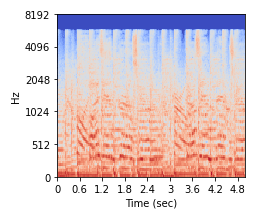
\includegraphics[width=2.5cm]{andr_mix.png}};
    \def\sourcea{0.25 * 2 * (0.5 * x - floor(0.5 * x))}
    \def\sourceb{0.25 * exp(-(x + 10)/10) * cos(deg(4 * x))}
    \def\sourcec{0.25 * cos(deg(0.3 * x)) * cos(deg(2 * x + 0.9 * cos(deg(4 * x)))}
    \def\sourced{0.25 * cos(deg(5 * x) * (
        1 + 0.1 * cos(deg(1 * x)))
     )}
    \node (wavplot) at (wav|-specimg) {};
    \begin{axis}[
        anchor=center,
        at=(wavplot),
        scale=0.6,
        domain=-10:10,
        axis y line=none,
        axis x line=none,
        samples=200,
        color=black,
        height=2.5cm,
        width=1.5 * \base]
          \addplot[mark=none] {
              (
                \sourcea + \sourceb + \sourcec + \sourced
               )
         };
    \end{axis}
    \node (istft) [shape=rectangle, fill=green!5, minimum width=0.5*\base,rounded corners=1pt,draw=black!90] at
        ($ (wavplot.west) + (-6cm, 0cm) $) {$\mathrm{STFT}$};
    \draw [->] ($(wavplot) + (-3cm, 0cm)$) -- (istft.east);
    \draw [->] (istft.west) -- (specimg.east);

    \node (e1) [conv, tbranch, minimum width=\base, anchor=south] at ($(wav.north) + (0, \yshift)$)
        {$\mathrm{TEncoder}_1(C_{in}=2, C_{out}=48)$};
    \node [tt, anchor=west] at ($ (e1.south) + (+0.1cm, -\yshift/2) $) {$T$ time steps};

    \node [tt,anchor=west] at ($(e1.north) + (0.1cm, \yshift/2)$) {T/4 time steps};

    \node (e2) [conv, tbranch, minimum width=\base - \dec, anchor=south] at ($(e1.north) + (0, \yshift)$)
        {$\mathrm{TEncoder}_2(C_{in}=48, C_{out}=96)$};
    \node [tt,anchor=west] at ($(e2.north) + (0.1cm, \yshift/2)$) {T/16 time steps};

    \node (e3) [conv, tbranch, minimum width=\base - 2*\dec, anchor=south] at ($(e2.north) + (0, \yshift)$)
        {$\ldots$};
    \node [tt,anchor=west] at ($(e3.north) + (0.1cm, \yshift/2)$) {T/256 time steps};

    \node (e5) [conv, tbranch, minimum width=\base - 3*\dec, anchor=south, inner ysep=2pt] at ($(e3.north) + (0, \yshift)$)
        {$\mathrm{TEncoder}_5(C_{in}=384, C_{out}=768)$};
    \node [tt,anchor=west] at ($(e5.north) + (0.1cm, \yshift/2)$) {T/1024 time steps};

    % Spec encoder

    \node (e1z) [conv, zbranch, minimum width=\base] at ($(spec.north) + (0, \yshift)$)
        {$\mathrm{ZEncoder}_1(C_{in}=2\cdot 2, C_{out}=48)$};

    \node [tt, anchor=west, align=left] at ($ (e1z.south) + (-0.7cm, -\yshift/2) $) {$T/1024$ time steps $2048$ freq.};

    \node [tt,anchor=west] at ($(e1z.north) + (-0.7cm, \yshift/2)$) {T/1024 time steps, 512 freq.};

    \node (e2z) [conv, zbranch, minimum width=\base - \dec] at ($(e1z.north) + (0, \yshift)$)
        {$\mathrm{ZEncoder}_2(C_{in}=48, C_{out}=96)$};
    \node [tt,anchor=west] at ($(e2z.north) + (-0.7cm, \yshift/2)$) {T/1024 time steps, 256 freq.};

    \node (e3z) [conv, zbranch, minimum width=\base - 2*\dec] at ($(e2z.north) + (0, \yshift)$)
        {$\ldots$};
    \node [tt,anchor=west] at ($(e3z.north) + (-0.7cm, \yshift/2)$) {T/1024 time steps, 8 freq.};

    \node (e5z) [conv, zbranch, minimum width=\base - 3*\dec, inner ysep=2pt] at ($(e3z.north) + (0, \yshift)$)
        {$\mathrm{ZEncoder}_5(C_{in}=384, C_{out}=768)$};
    \node [tt,anchor=west] at ($(e5z.north) + (-0.7cm, \yshift/2)$) {T/1024 time steps, 1 freq.};

    \node (merge) [circle,draw=black, inner sep=1pt,fill=black!5] at ($ (base |- e5z.north) + (0, 0.5*\yshift)$) {\huge $+$};

    \draw[->] (e5z.east) -- (merge.west);
    \draw[->] (e5.west) -- (merge.east);

    \node (share) [conv, sbranch, minimum width=\base + 2 *\dec] at ($ (merge.north) + (0, 0.5*\yshift)$) {$\mathrm{Encoder}_6(C_{in}=768, C_{out}=1586)$};

    \draw[->] (merge.north) -- (share.south);

    \node [tt,anchor=west] at ($(share.north) + (1cm, \yshift/2)$) {T/2048 time steps};

    \node (shared) [deconv, sbranch, minimum width=\base + 2*\dec] at ($ (share.north) + (0, \yshift)$) {$\mathrm{Decoder}_6(C_{in}=1586, C_{out}=768)$};
    \node [tt,anchor=west] at ($(shared.north) + (1cm, \yshift/2)$) {T/1024 time steps};

    % decoder Z
    \node (d5z) [deconv, zbranch, minimum width=\base - 3 * \dec, inner ysep=2pt] at
        ($ (e5z.north |- shared.north) + (0, \yshift) $)
        {$\mathrm{ZDecoder}_5(C_{in}=768, C_{out}=386)$};
    \node [tt,anchor=west] at ($(d5z.north) + (-0.7cm, \yshift/2)$) {T/1024 time steps, 8 freq.};
    \node (d4z) [deconv, zbranch, minimum width=\base - 2 * \dec] at
        ($ (d5z.north) + (0, \yshift) $)
        {$\ldots$};
    \node [tt,anchor=west] at ($(d4z.north) + (-0.7cm, \yshift/2)$) {T/1024 time steps, 256 freq.};
    \node (d2z) [deconv, zbranch, minimum width=\base - \dec] at
        ($ (d4z.north) + (0, \yshift) $)
        {$\mathrm{ZDecoder}_2(C_{in}=96, C_{out}=48)$};
    \node [tt,anchor=west] at ($(d2z.north) + (-0.7cm, \yshift/2)$) {T/1024 time steps, 512 freq.};
    \node (d1z) [deconv, zbranch, minimum width=\base] at
        ($ (d2z.north) + (0, \yshift) $)
        {$\mathrm{ZDecoder}_2(C_{in}=48, C_{out}=4 \cdot 2 \cdot 2)$};
    \node [tt,anchor=west] at ($(d1z.north) + (-0.7cm, \yshift/2)$) {T/1024 time steps, 2048 freq.};

    \node [anchor=south] at ($ (d1z) + (-3cm, \yshift) $) {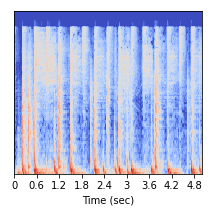
\includegraphics[width=2cm]{andr_drums.png}};
    \node [anchor=south] at ($ (d1z) + (-1cm, \yshift) $) {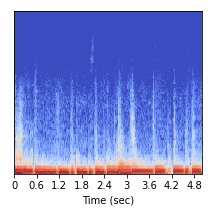
\includegraphics[width=2cm]{andr_bass.png}};
    \node [anchor=south] at ($ (d1z) + (1cm, \yshift) $) {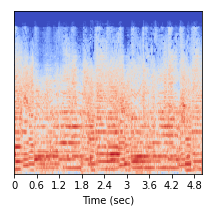
\includegraphics[width=2cm]{andr_other.png}};
    \node [anchor=south] at ($ (d1z) + (3cm, \yshift) $) {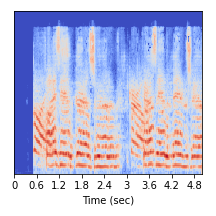
\includegraphics[width=2cm]{andr_vocals.png}};
    \node (istft) [shape=rectangle, fill=green!5, minimum width=\base,rounded corners=1pt,draw=black!90] at
        ($ (d1z.north) + (0, 3cm) $) {$\mathrm{ISTFT}$};


    % decoder T
    \node (d5t) [deconv, tbranch, minimum width=\base - 3 * \dec, inner ysep=2pt] at
        ($ (e5.north |- shared.north) + (0, \yshift) $)
        {$\mathrm{TDecoder}_5(C_{in}=768, C_{out}=386)$};
    \node [tt,anchor=west] at ($(d5t.north) + (0.1cm, \yshift/2)$) {T/1024 time steps};
    \node (d4t) [deconv, tbranch, minimum width=\base - 2 * \dec] at
        ($ (d5t.north) + (0, \yshift) $)
        {$\ldots$};
    \node [tt,anchor=west] at ($(d4t.north) + (0.1cm, \yshift/2)$) {T/256 time steps};
    \node (d2t) [deconv, tbranch, minimum width=\base - \dec] at
        ($ (d4t.north) + (0, \yshift) $)
        {$\mathrm{TDecoder}_2(C_{in}=96, C_{out}=48)$};
    \node [tt,anchor=west] at ($(d2t.north) + (0.1cm, \yshift/2)$) {T/4 time steps};
    \node (d1t) [deconv, tbranch, minimum width=\base] at
        ($ (d2t.north) + (0, \yshift) $)
        {$\mathrm{TDecoder}_1(C_{in}=48, C_{out}=4 \cdot 2 \cdot 2)$};
    \node [tt,anchor=west] at ($(d1t.north) + (0.1cm, \yshift/2)$) {T time steps.};

    \node (merge2) [circle,draw=black, inner sep=1pt,fill=black!5] at (istft -| d1t.north) {\huge $+$};
    \draw [->] (istft.east) -- (merge2.west);
    \draw [->] (d1t.north) -- (merge2.south);


    \newcommand\myoutput[3]{
        \begin{axis}[
            anchor=south,
            scale=0.6,
            at=#1,
            domain=-20:20,
            axis y line=none,
            axis x line=none,
            samples=200,
            height=2.5cm,
            color=#2,
            width=3 * \base]
            \addplot[mark=none] {
                #3
            };
        \end{axis}
    }
    \node (o1) [yshift=\yshift] at (istft.north -| merge) {};
    \node (o2) at ($(o1.north) + (0, 4mm)$) {};
    \node (o3) at ($(o2.north) + (0, 4mm)$) {};
    \node (o4) at ($(o3.north) + (0, 4mm)$) {};
    \myoutput{(o1)}{violet}{\sourcea}
    \myoutput{(o2)}{olive}{\sourceb}
    \myoutput{(o3)}{red}{\sourcec}
    \myoutput{(o4)}{blue}{\sourced}

    \path[skip] (e1.east) edge[bend right=15] node [right] {} (d1t.east);
    \path[skip] (e2.east) edge[bend right=15] node [right] {} (d2t.east);
    \path[skip] (e3.east) edge[bend right=15] node [right] {} (d4t.east);
    \path[skip] (e5.east) edge[bend right=15] node [right] {} (d5t.east);

    \path[skip] (e1z.west) edge[bend left=15] node [left] {} (d1z.west);
    \path[skip] (e2z.west) edge[bend left=15] node [left] {} (d2z.west);
    \path[skip] (e3z.west) edge[bend left=15] node [left] {} (d4z.west);
    \path[skip] (e5z.west) edge[bend left=15] node [left] {} (d5z.west);
  \end{tikzpicture}

\end{document}